\section{Quellen}

\begin{tabular}{ll}
    Thévenin    & Spannungsquelle mit Seriewiderstand \\
    Norton      & Stromquelle mit Parallelwiderstand
\end{tabular}

\vspace{0.1cm}

\crd{\textbf{ \textrightarrow\ DC- und AC-Signale werden separat betrachtet!} }


\subsection{Superpositionsprinzip}

Eingangssignale eines \textbf{linearen Netzwerks} dürfen separat betrachtet werden. \\
(nur eine Quelle aktiv, die anderen Quellen werden ausgeschaltet)

\vspace{0.1cm}

\textbf{ \textrightarrow\ Superpositionsprinzip funktioniert nicht in der Sättigung!}


\section{Grundlagen}

\subsection{Kleinsignal-Ersatzschaltung (!)}
\label{kleinsignal-ersatzschlatung}

\textbf{Ziel:} Berechnung der \textbf{AC-Spannungen} an den verschiedenen Knoten der Schaltung sowie der Wechselströme in allen 
Zweigen der Schaltung.

\vspace{0.1cm}

\begin{itemize}
    \item DC-Spannungsquellen durch Kurzschlüsse ersetzen
    \item DC-Stromquellen entfernen (Unterbrüche)
    \item Nichtlineare Bauteile mit Kleinsignal-Ersatzschlatung ersetzen
    \item Koppel- und Bypass-Kondensatoren kurzschliessen
    \item Spulen entfernen
\end{itemize}


\subsection{Schaltungsanalyse - Vorgehen (!)}

\textbf{DC-Arbeitspunkte und Verstärkungsfaktor bestimmen}

\vspace{0.1cm}

\begin{itemize}
    \item Arbeitspunkte bestimmen (DC-Spannung in jedem Knoten)
    \item Kleinsignalersatzschaltung gemäss Kapitel \ref{kleinsignal-ersatzschlatung} bilden
    \item Schaltung ggf. umzeichnen und vereinfachen
    \item Verstärkung $\frac{V_{\rm out}}{V_{\rm in}}$ berechnen 
\end{itemize}


\subsection{Dezibel}

\vspace{-0.2cm}

\begin{center}
    \renewcommand{\arraystretch}{2}
    \begin{tabular}{c c c}
        \myul{\textbf{Dezibel}}                                                                                             &               & \myul{\textbf{Faktor}}                                \\
        $A_{\deci \bel}  = 20 \log \Biggl( \Bigl|\underbrace{\frac{V_{\rm out}}{V_{\rm in}}}_{\substack{A}} \Bigr| \Biggr)$ & \textlrarrow\ & $A  = 10^{\frac{A_{\deci \bel}}{20 \, \deci \bel}}$   \\
        $A_{\rm total} = A_{\deci \bel 1} + A_{\deci \bel 2}$                                                               &               & $A_{\rm total} = A_1 \cdot A_2$                       
    \end{tabular}
    \renewcommand{\arraystretch}{1}
\end{center}


\section{Verstärker}

\subsection[Übertragungsfaktor (reale Verstärker)]{Übertragungsfaktor $\bm{k}$ (reale Verstärker)}

\begin{center}
    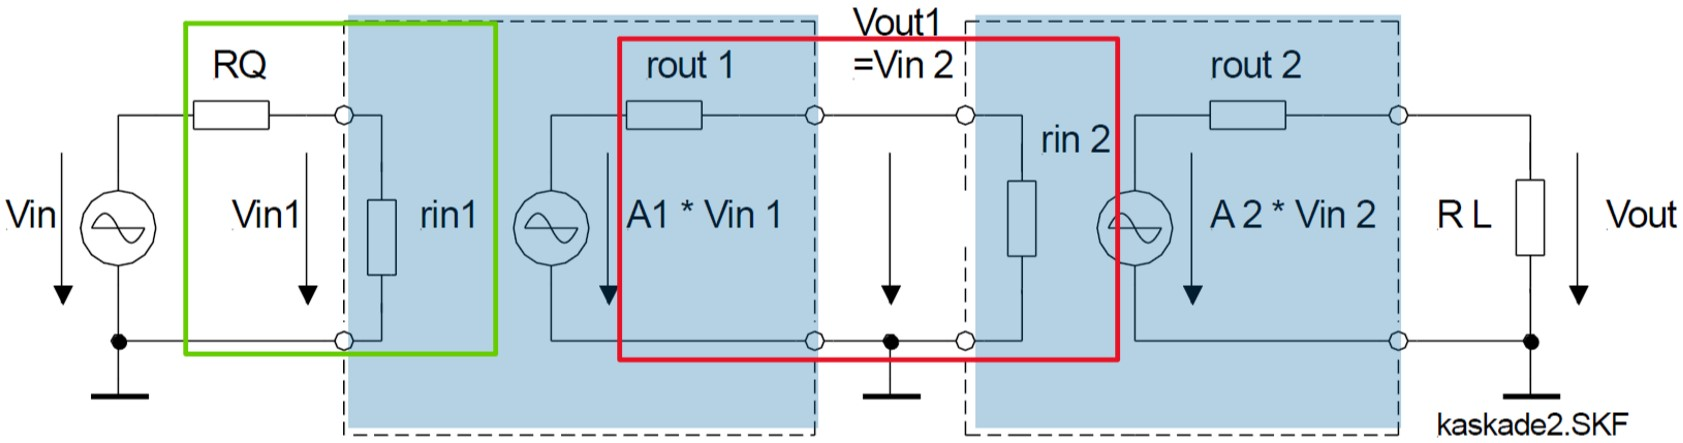
\includegraphics[width=0.75\columnwidth]{images/kopplungsfaktor.jpg}
\end{center}

\begin{tabular}{lll}
    $ V_{\rm in1} = V_{\rm in} \cdot \cgn{ \underbrace{ \frac{R_{\rm in1}}{R_{\rm in1} + R_Q} }_{\substack{k_1}} } $            &
    $ V_{\rm in2} = \crd{\underbrace{ \frac{R_{\rm in2}}{R_{\rm in2} + R_{\rm out1}} }_{\substack{k_2}} } \cdot V_{\rm out1} $  &
    $ V_{\rm out} = V_{\rm in} \cdot k_1 \cdot A_1 \cdot k_2 \cdot A_2 \cdot k_L $
\end{tabular}

